\chapter{Automotive - State of art}

Self driving cars are one of the hottest topics of the decade. Artificial Intelligences specifically trained to drive with machine learning techniques demonstrated that it's possible for a computer to drive cars. However, a failure of these systems may have very serious consequences that could result in people being injuried, or killed. At the same time, it is a problem to certify the ultra-high dependability requirements demanded. In this chapter, today's problems regarding the safety issues related to self driving cars are reviewed, for that it was decided to conduct this study.

\section{Autonomous Cars as CPS}

In order for a car to be able to drive by itself, suitable hardware and software are required. This makes autonomous cars cyber physical systems, and the possible catastrophic consequences that a failure in/of these systems can cause, make them fall under the set of critical systems.

To sense and map the surrounding environment, the system collects data from multiple sensors. Some of the most important sensors and their purposes are listed here:

\begin{itemize}
	\item GPS
	\begin{itemize}
		\item[$\rightarrow$] High precision GPS sensors are used to estimate the exact position on the vehicle in the world
	\end{itemize}
	\item Odometry \& IMU sensors
	\begin{itemize}
		\item[$\rightarrow$] These sensors are worth for detecting changes in the position of the car and of the objects in the environment over time
	\end{itemize}
	\item Cameras
	\begin{itemize}
		\item[$\rightarrow$] Cameras are literally the \textsl{eyes} of the system. Images captured are usually processed with image recognition software
	\end{itemize}
	\item Lidars \& Radars
	\begin{itemize}
		\item[$\rightarrow$] Lidars can be seen as the evolution of conventional radars. Data combined from these sensors serve the purpose of mapping the environment and detect obstacles and objects around the car
	\end{itemize}
\end{itemize}

Outputs from these sensors are combined and given to the car's control system.
An abstraction of the software architecture is shown in this figure:
\vspace{-1cm}
\begin{figure}[h!]
	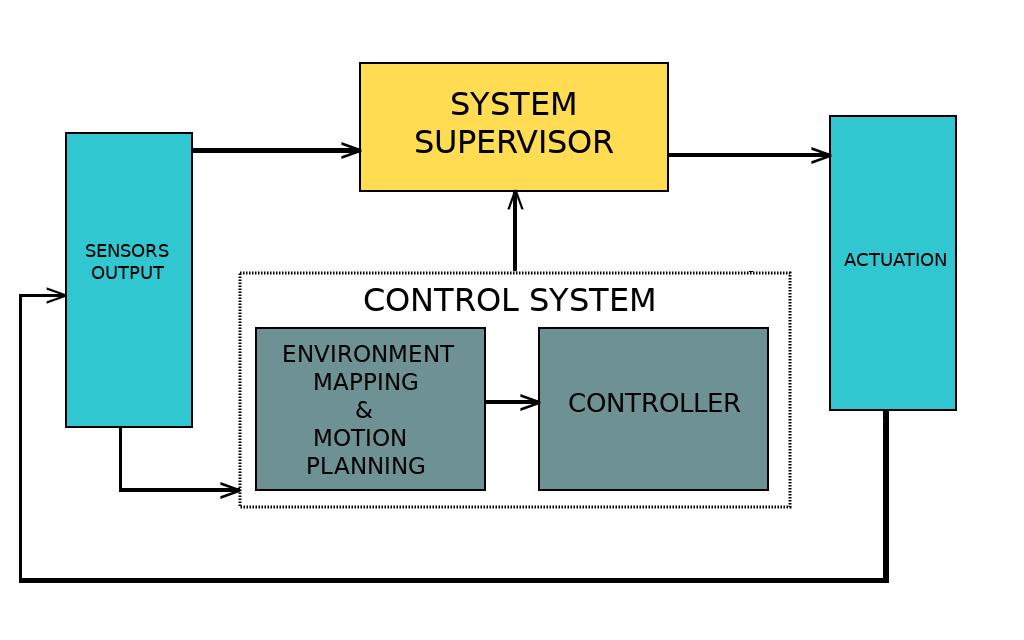
\includegraphics[width=\textwidth]{img/av-architecture.png}
	\caption{High-level abstraction of the system's software architecture}
\end{figure}

Data from sensors are inputs of the control system, here simplified as composed by two constituent systems: one in charge of collecting data directly from the sensors, process them in order to build an \textsl{occupancy grid}\footnote{A matrix mapping the environment, the cells $a_{i,j}$ are flagged with 0 if there's no object at coordinates $i,j$, 1 if occupied.} to map the surrounding area and to create a physical model of the environment in order to follow the correct route to the destination without crashing. The Controller (usually composed as a combination of a Velocity Controller\footnote{Controller in charge of adjusting the vehicle's speed} and a Steering Controller\footnote{Controller that determines the steering angle}) uses these data to adjust the values on the actuators controlling the movements of the car: throttle, brake and steer.\newline
Due to the criticity of their task, it's mandatory to have a System Supervisor, a System in charge of detecting possible hardware failures or wrong outputs\footnote{With \textsl{"wrong"} is intended not only outputs out of the domain space but also outputs that would cause the system to fail (e.g. causing a crash)} from the Control System and, if needed, activate a corrective routine.

The System Supervisor is the main failure avoidance component of such systems. Of course there may be specific checks when data are processed, but the last decision is up to this system's monitor and the underestimation of its importance can lead to dramatic consequences, such as the 2018 accident in Arizona, where a woman was killed by a self-driving car during a test run.\cite{arizuber} Further inspections showed that the car's radar and LiDAR sensors detected the victim almost 6 seconds before the impact and it took 4 seconds circa to infer that there was an obstacle on the road and that an emergency brake was needed. However, this safety-checker was disabled during tests for "smoother rides", causing the accident.\cite{govarizuber}\newline\newline
The extreme complexity of these systems raise concerns among the experts: the need to find a new point of view to study and test the safety of these systems, and the need to sensitise about safety culture.\cite{koopman}


\section{Safety And Autonomous Vehicles}

According to a SAE International tentative to classify self-driving cars' autonomy, the level of automation can be divided in 6 tiers, ranging from 0 to 5. Level 0 means no autonomy: a human driver just drives the car; level 5 means that there's no need of human intervention at all and the car is not only capable of driving safely on the road, but it must be able to avoid catastrophic failures that may seriously harm (or kill) people.
The more autonomous the car is, the higher the dependability requirements are for it to be put on public roads.
It is a well known issue that demonstrating a system's dependability is not an easy task for itself, it gets even harder with ultra-high dependability systems such as these are. In adition to the problem itself, demonstrating autonomous cars' dependability has two more problems to deal with: how to safely and effectively test the system and the presence of neural networks, for which it's very hard to understand why it returned the output $y$, given the input $x$.

Lots of studies demonstrated that it's unthinkable to just test cars on the roads. One of these, that we will refer to as the RAND Study, answers the question of how many miles of driving would it take to demonstrate autonomous vehicles' reliability using classical statistical inference, saying that if autonomous cars fatality rate was 20\% lower than humans', it would take more than 500 years with \textsl{"a fleet of 100 autonomous vehicles being test-driven 24 hours a day, 365 days a year at an average speed of 25 miles per hour"}.\cite{randstudy}\newline
The validation of ultra-high dependability requirements for safety-critical systems is a well known problem in safety literature and has not been introduced by the advent of autonomous cars. In fact, the RAND study is nothing but a specific case of the problem considered in a work published in 1993 by Littlewood \& Strigini, in which the same concepts are discussed and generalized for every ultra-high dependability system.\cite{littlewoodStrigini}\newline
The main problem with the RAND study approach is that future failures frequency can not be predicted just using the observed one. Not just for the quantitative results of the impossibility of it, but also because this approach can not work: an observed frequency failure of $0$ would lead to optimistic (and probably harmful) predictions. Luckily, this problem is surmountable, as shown in \textsl{this}\cite{zhaoStrigini} work by Zhao et al.

Validating the dependability requirements of an autonomous car seems a hard task already. Things are made even harder by the fact that these cars are driven by neural networks.\newline
In these years there is a huge growing interest in the \textsl{machine learning} sector, and this has made that a lot of progress was done in the research. It's also thanks to these progresses that autonomous cars now seem like something we can achieve, since these AIs gave surprising results with their skills, and big brands such as \textsl{Uber} and \textsl{Tesla} are putting more and more efforts in AI research.
This new wave of AI research is deeply changing the way we interact with computer systems, and surprising results were achieved with neural networks.\newline
These tools have proven to outclass \textsl{"classic"} software solutions (intended as non-neural network) in a lot of tasks, ranging from \textsl{Object Detection}\cite{retinaNet} to \textsl{Gaming}\cite{alphaGo} problems, performing even better than humans.\cite{alphaGoBeatsMan}
The complexity of the environment in which the system performs and the need of quick decision-making procedures and fast responses to events that \textsl{cannot} be planned with \textsl{"classic"} software, make neural networks the perfect tool to achieve the task of a car being able to drive by itself, thanks to their ability to handle multiple situations that were not explicitly written in the software. However, this raises serious issues about the safety of the whole system for many reasons.\newline

If neural networks gave promising results on one hand, and they seem the only way to achieve goals such as autonomous cars, on the other hand it has been shown many times how weird a network's prediction can get when \textsl{minimally} perturbating the inputs\cite{stupidnn} and how high the confidence interval can be.\cite{foolnn} The lack of official regulations and certifications for this kind of software, as well as the need to truly understand neural networks, is raising concerns on how dependable these systems can be and consciousness is now growing on the topic, asking for more regulations on companies developing advanced AIs.\cite{elonmusk}

\section{Controller - Checker Problem}


The interaction between the Control System and the System Supervisor is at the core of the car's movements. The Control System, or \textsl{Primary Component}, is the software performing the main computations of the system, required to drive the car. In a context like this, it's mandatory to have fault-tolerance mechanisms such as the System Supervisor, to avoid catastrophic failures. This kind of architecture is a must for these systems, due to the extremely high dependability requirements they have, in order to try to cover all the possible failures that may happen. The state space of such systems may be sketched as in figure 7.
\vspace{0.3cm}
\begin{figure}[h!]
	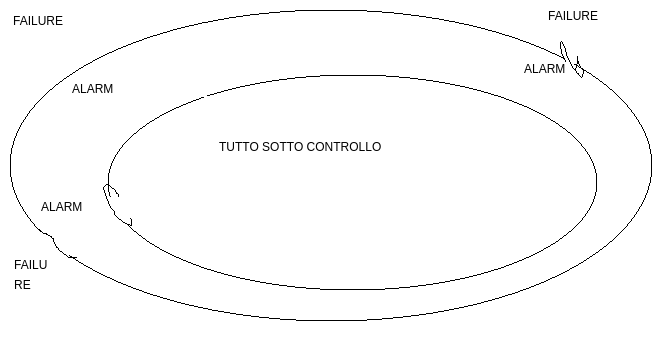
\includegraphics[width=\textwidth,height=7.3cm]{img/state-space.png}
	\caption{Sketch of the system's safe states}
\end{figure}
\newpage

We consider \textsl{safe states} all the states in which the Control System produces an output that would not result in a crash.
If we model the system's failures in this way, the level of safety of the system can be represented as the union of the failure area covered by the Controller and the one covered by the Supervisor, with an \textsl{overlap area} in which the Supervisor is actually \textsl{detrimental} to the System performances.

Now imagine that an autonomous car is riding when suddenly an obstacle appears. If the Primary correctly detects the obstacles it should autonomously apply a safety-measure to \textbf{avoid} a transition in an \textsl{alert state}. If the controller doesn't see the obstacle, \textsl{or} detects it but keeps throttling we say that the Controller is \textsl{failed} and there is a transition from a \textsl{safe-state} to an \textsl{alert-state}, in which the failure-avoidance components turn in. The System Supervisor's duty is now to launch a corrective-routine that will put the system in a fail-safe state (e.g. by applying the safety-brake and turning off the engine). An error of the Supervisor will inevitably cause the system to fail, as a result of the failure of both components, leading in a failure state (the crash happened). 

The possible behaviours of the System Supervisor can be represented using the \textsl{Confusion Matrix}, a specific table layout that allows visualization of the performance of a \textsl{classification algorithm}.\cite{wikiconfmatrix}\newline
This special kind of \textsl{contingency table} has two dimensions: \textsl{actual value} and \textsl{predicted value}:

\vspace{0.5cm}

\begin{tabular}{l|l|c|c|c}
	\multicolumn{2}{c}{}&\multicolumn{2}{c}{Actual Value}&\\
	\cline{3-4}
	\multicolumn{2}{c|}{}&Positive&Negative& \\
	\cline{2-4}
	\multirow{2}{*}{Predicted Value}& Positive & $TP$ & $FP$ & \\
	\cline{2-4}
	& Negative & $FN$ & $TN$ & \\
	\cline{2-4}
\end{tabular}

\vspace{0.8cm}

Recall that what we defined a \textsl{"failure"} of the Controller as a transition from a \textsl{safe state}: a state in which the Controller can handle what's happening in the environment without crashing, to an \textsl{alert state}: a condition in which without the Supervisor, the System would inevitably go in a failure state.
For this component, we want to measure its ability to distinguish between safe states and alert states. To do so, we defined positives and negatives predictions in this way:

\begin{itemize}
	\item[TP:] True Positive
	\begin{itemize}
		\item[-] The system went in an alert state due to a Controller's failure, correctly detected and prevented by the monitor
	\end{itemize}
	\item[TN:] True Negative
	\begin{itemize}
		\item[-] The system is in a safe state and the Monitor doesn't raise any alarm
	\end{itemize}
	\item[FP:] False Positive
	\begin{itemize}
		\item[-] The system is in a safe state, but the Monitor raises an alarm
	\end{itemize}
	\item[FN:] False Negative
	\begin{itemize}
		\item[-] The system is in an alert state and the Monitor doesn't detect the hazard
	\end{itemize}
\end{itemize}


\begin{figure}[h!]
	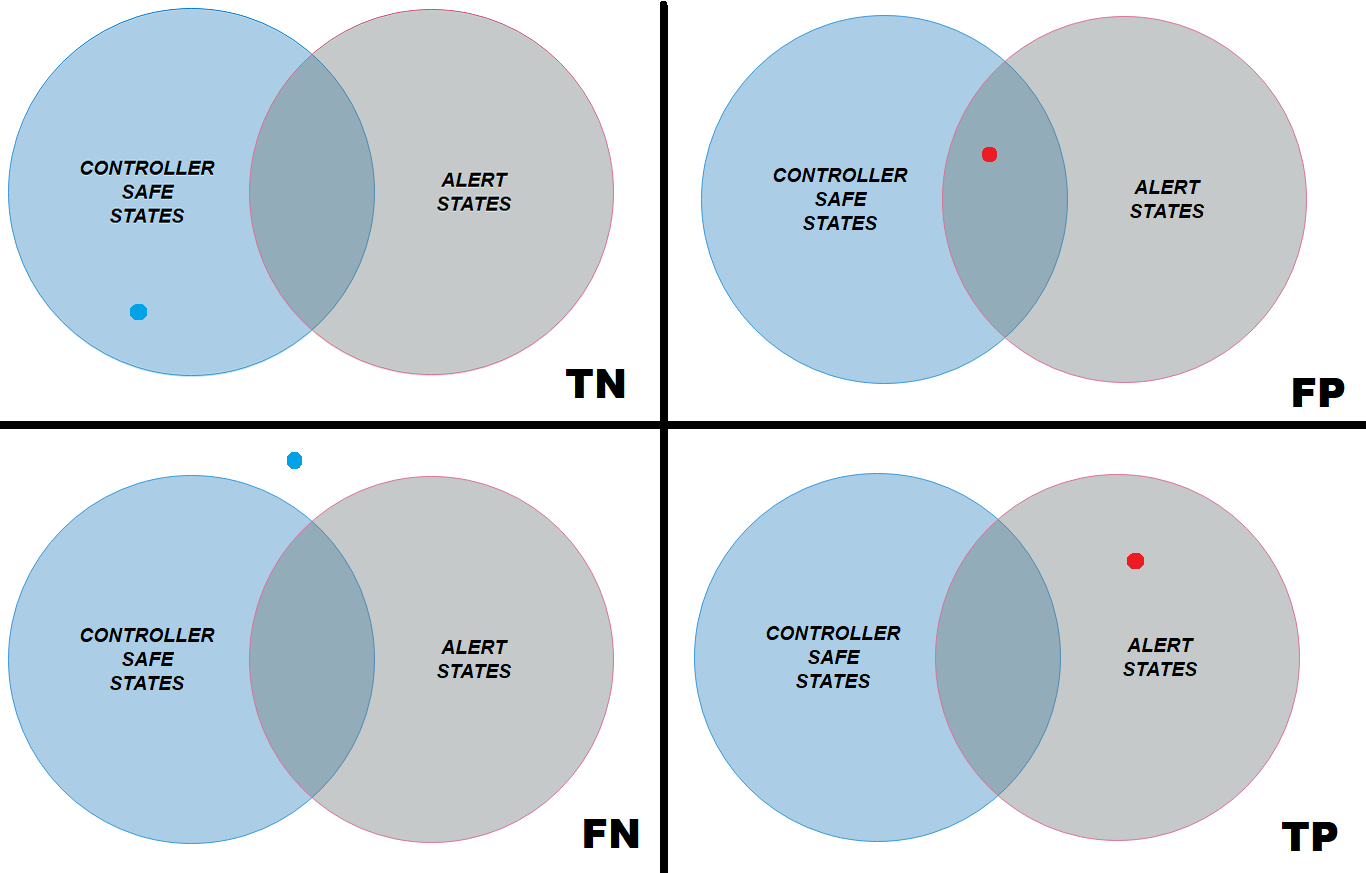
\includegraphics[width=\textwidth]{img/positive-negative-set.png}
	\caption{Graphical Representation of what true and false predictions means in the system's state space. Dots represent the current state of the System. A blue dot means that no alarm is raised, a red dot means that the Monitor raises an alarm}
\end{figure}

\vspace{0.5cm}

These raw values are nothing but a starting point to compute more complex and meaningful measures, usually presented in form of \textsl{rates}, linked with each other using statistical laws, making them equivalent from a statistical point of view and easy to compute once the amounts of correct/wrong predictions are known. Examples of some of these measures are:

\begin{itemize}
	\item \textsl{Sensitivity (True Positive Rate):} measures the proportion of actual positives, correctly identified as such
	\begin{itemize}
		\item[] $TPR = \frac{TP}{TP+FN} = 1-FNR$
	\end{itemize}
	\item \textsl{Specificity (True Negative Rate):} measures the proportion of actual negatives, correctly identified as such
	\begin{itemize}
		\item[] $TNR = \frac{TN}{TN+FP} = 1-FPR$
	\end{itemize}
	\item \textsl{Miss Rate (False Negative Rate):} measures the proportion of actual positives predicted as negatives
	\begin{itemize}
		\item[] $FNR = \frac{FN}{FN+TN} = 1-TPR$
	\end{itemize}
	\item \textsl{Fall-out (False Positive Rate):} measures the proportion of actual negatives predicted as positives
	\begin{itemize}
		\item[] $FPR = \frac{FP}{FP+TN} = 1-TNR$
	\end{itemize}
\end{itemize}

These four rates can be combined as well, to approximate the \textsl{Accuracy} and \textsl{Precision} of our predictions:

\begin{itemize}
	\item \textsl{Accuracy:} a measures used for describing \textsl{systematic errors} in predictions. A low \textsl{Accuracy} is the cause of differences between a prediction and its \textsl{"true"} value. ISO has defined this measure as an indicator of the \textsl{trueness} of predictions (i.e. the ability to predict \textsl{true values}) \cite{isoacc}
	\begin{itemize}
		\item[] $ACC = \frac{TP+TN}{TP+TN+FP+FN}$
	\end{itemize}
	\item \textsl{Precision:} a measures used for describing \textsl{random errors} in predictions, that is: a measure of \textsl{statistical variability} in the model used for predictions.
	\begin{itemize}
	\item[] $PREC = \frac{TP}{TP+FP}$
	\end{itemize}
\end{itemize}

It is important to keep in mind that once the amounts of correct and wrong predictions are known, all these measures can be computed (and many more, depending on the need of the case study) and linked to each other, making easy to switch point of view of the analysis.\newline

This problem is nothing but a generalization (related to safety) of the asymmetric fault-tolerant architecture for computer systems: the idea of having a \textsl{Primary Component} that performs the main computations, and a \textsl{Primary Checker} in charge of detecting (and correcting) possible errors of the Primary.\newline
The problem of assessing the dependability of these simpler (but still complex) systems is a well known topic in literature and was explored in different studies. In a relatively recent work published by \textsl{Popov} and \textsl{Strigini} in 2010, it is shown that the probability of a system failing on a specific input (or set of inputs), strictly depends on both the coverage of the Primary \textsl{and} the Primary Checker, as shown in the figure 7.\cite{striginiPopov}

In the context of self-driving cars we want the area covered by the primary to be the largest possible. This is done by intensive training of the neural networks that will control the car. As long as the network is trained \textsl{"properly"}, the control system should be able to handle most of the dangerous situations that may happen. At one point, it is possible that the Controller learns to handle the \textsl{"alert states"} covered by the System Supervisor, reducing the overall contribution to the system's safety given by the latter.

\begin{figure}[h!]
	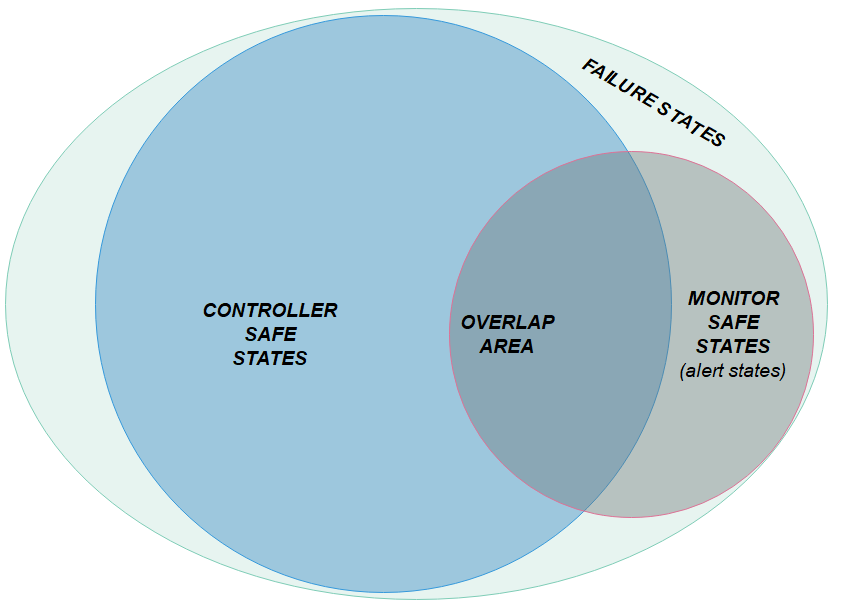
\includegraphics[width=\textwidth]{img/area-growth-good.png}
	\caption{The states covered by the Controller are now the ones previously covered, plus some states previously covered just by the Monitor}
\end{figure}

Another possibility is that during the training, a portion of the failure area covered by the controlller becomes uncovered. This could result in a situation in which some of the previously safe states are now alarm state, representing a serious harm to the system's dependability. Since the coverage area provided by the System Supervisor can not change without changing its implementation (it doesn't "learn" automatically), a transition to one of these states would now inevitably result in a failure.

\begin{figure}[h!]
	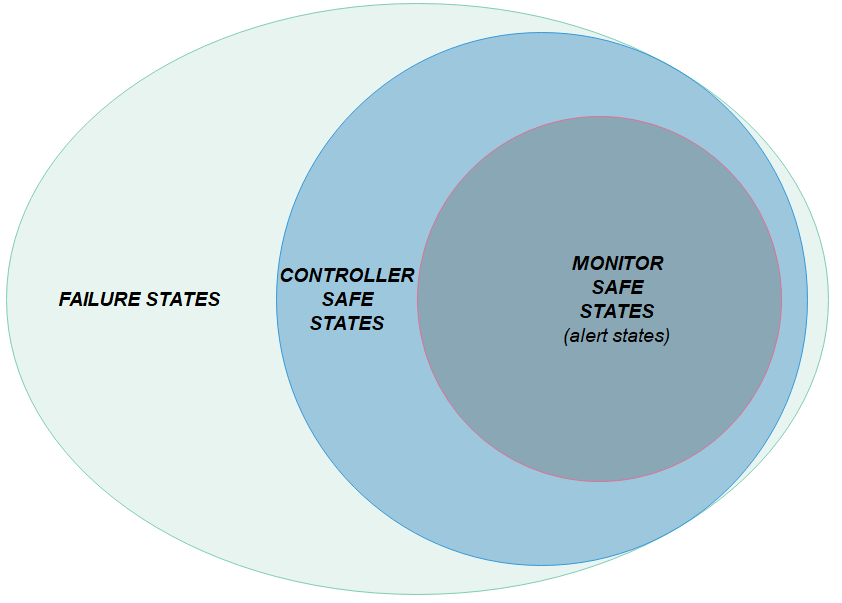
\includegraphics[width=\textwidth]{img/area-growth-bad.png}
	\caption{The Controller now covers all the states previously covered by the Monitor, but doesn't cover anymore some of the states he covered before the training}
\end{figure}

All these considerations and the lack of literature on the topic for these new systems such as autonomous cars, lead us to begin a study on the emergent behaviour resulting from the interaction of a neural network control system and a \textsl{"classic"} error checker, on what happens when the network is \textsl{taught} by a supervisor during the training and how performance metrics of these 2 components can be computed.\newline

In the next sections we present and discuss the development and implementation of an experimental methodology to study these aspects.

